\externaldocument{main.tex}
The application can be split into three distinct parts from a technological/architectural point of view:
\begin{itemize}
    \item The back-end API used to fetch and save data.
    \item The front-end part using Angular\parencite{angularDocs}.
    \item The Electron part used to deploy the application and to offer offline functionality.
  \end{itemize}
The back-end uses a MongoDB \parencite{mongoDocs} database to persist data. 
The decision to choose MongoDB was taken because of the use
case: A time keeping application needs to be highly flexible.
Entities such as projects and customers and the general company structure and therefore evolving requirements can change over time, 
possibly necessitating a different database structure. 
Due to MongoDB being a No-SQL database based on a JSON-like document structure, future changes regarding documents (which are analogous to tables 
in relational databases) require no changes to the database itself.
Such flexibility would greatly increase the future proofing of such an application.\paragraph{}
The back-end logic is developed in Python and uses the Flask framework \parencite{flaskDocs} for handling
requests from the front-end.
As mentioned previously for each entity (project, customer, template, and entry) there is business
logic to support create, update, and remove operations.\paragraph{}
The front-end uses Angular \parencite{angularDocs} and Angular Material \parencite{angularMaterialDocs}.
Angular was chosen as it is a very popular framework for single page applications and furthermore,
it makes it easy to develop re-usable UI components.
As for the components library, Angular Material was used because of its ease of use and well-known design, 
meaning users can easily adjust to the new user interface.
\begin{figure}[H]
  \centering
  \label{fig:pze-class-diagram}
  \caption{A class diagram representing all entities, relationships and operations.}
  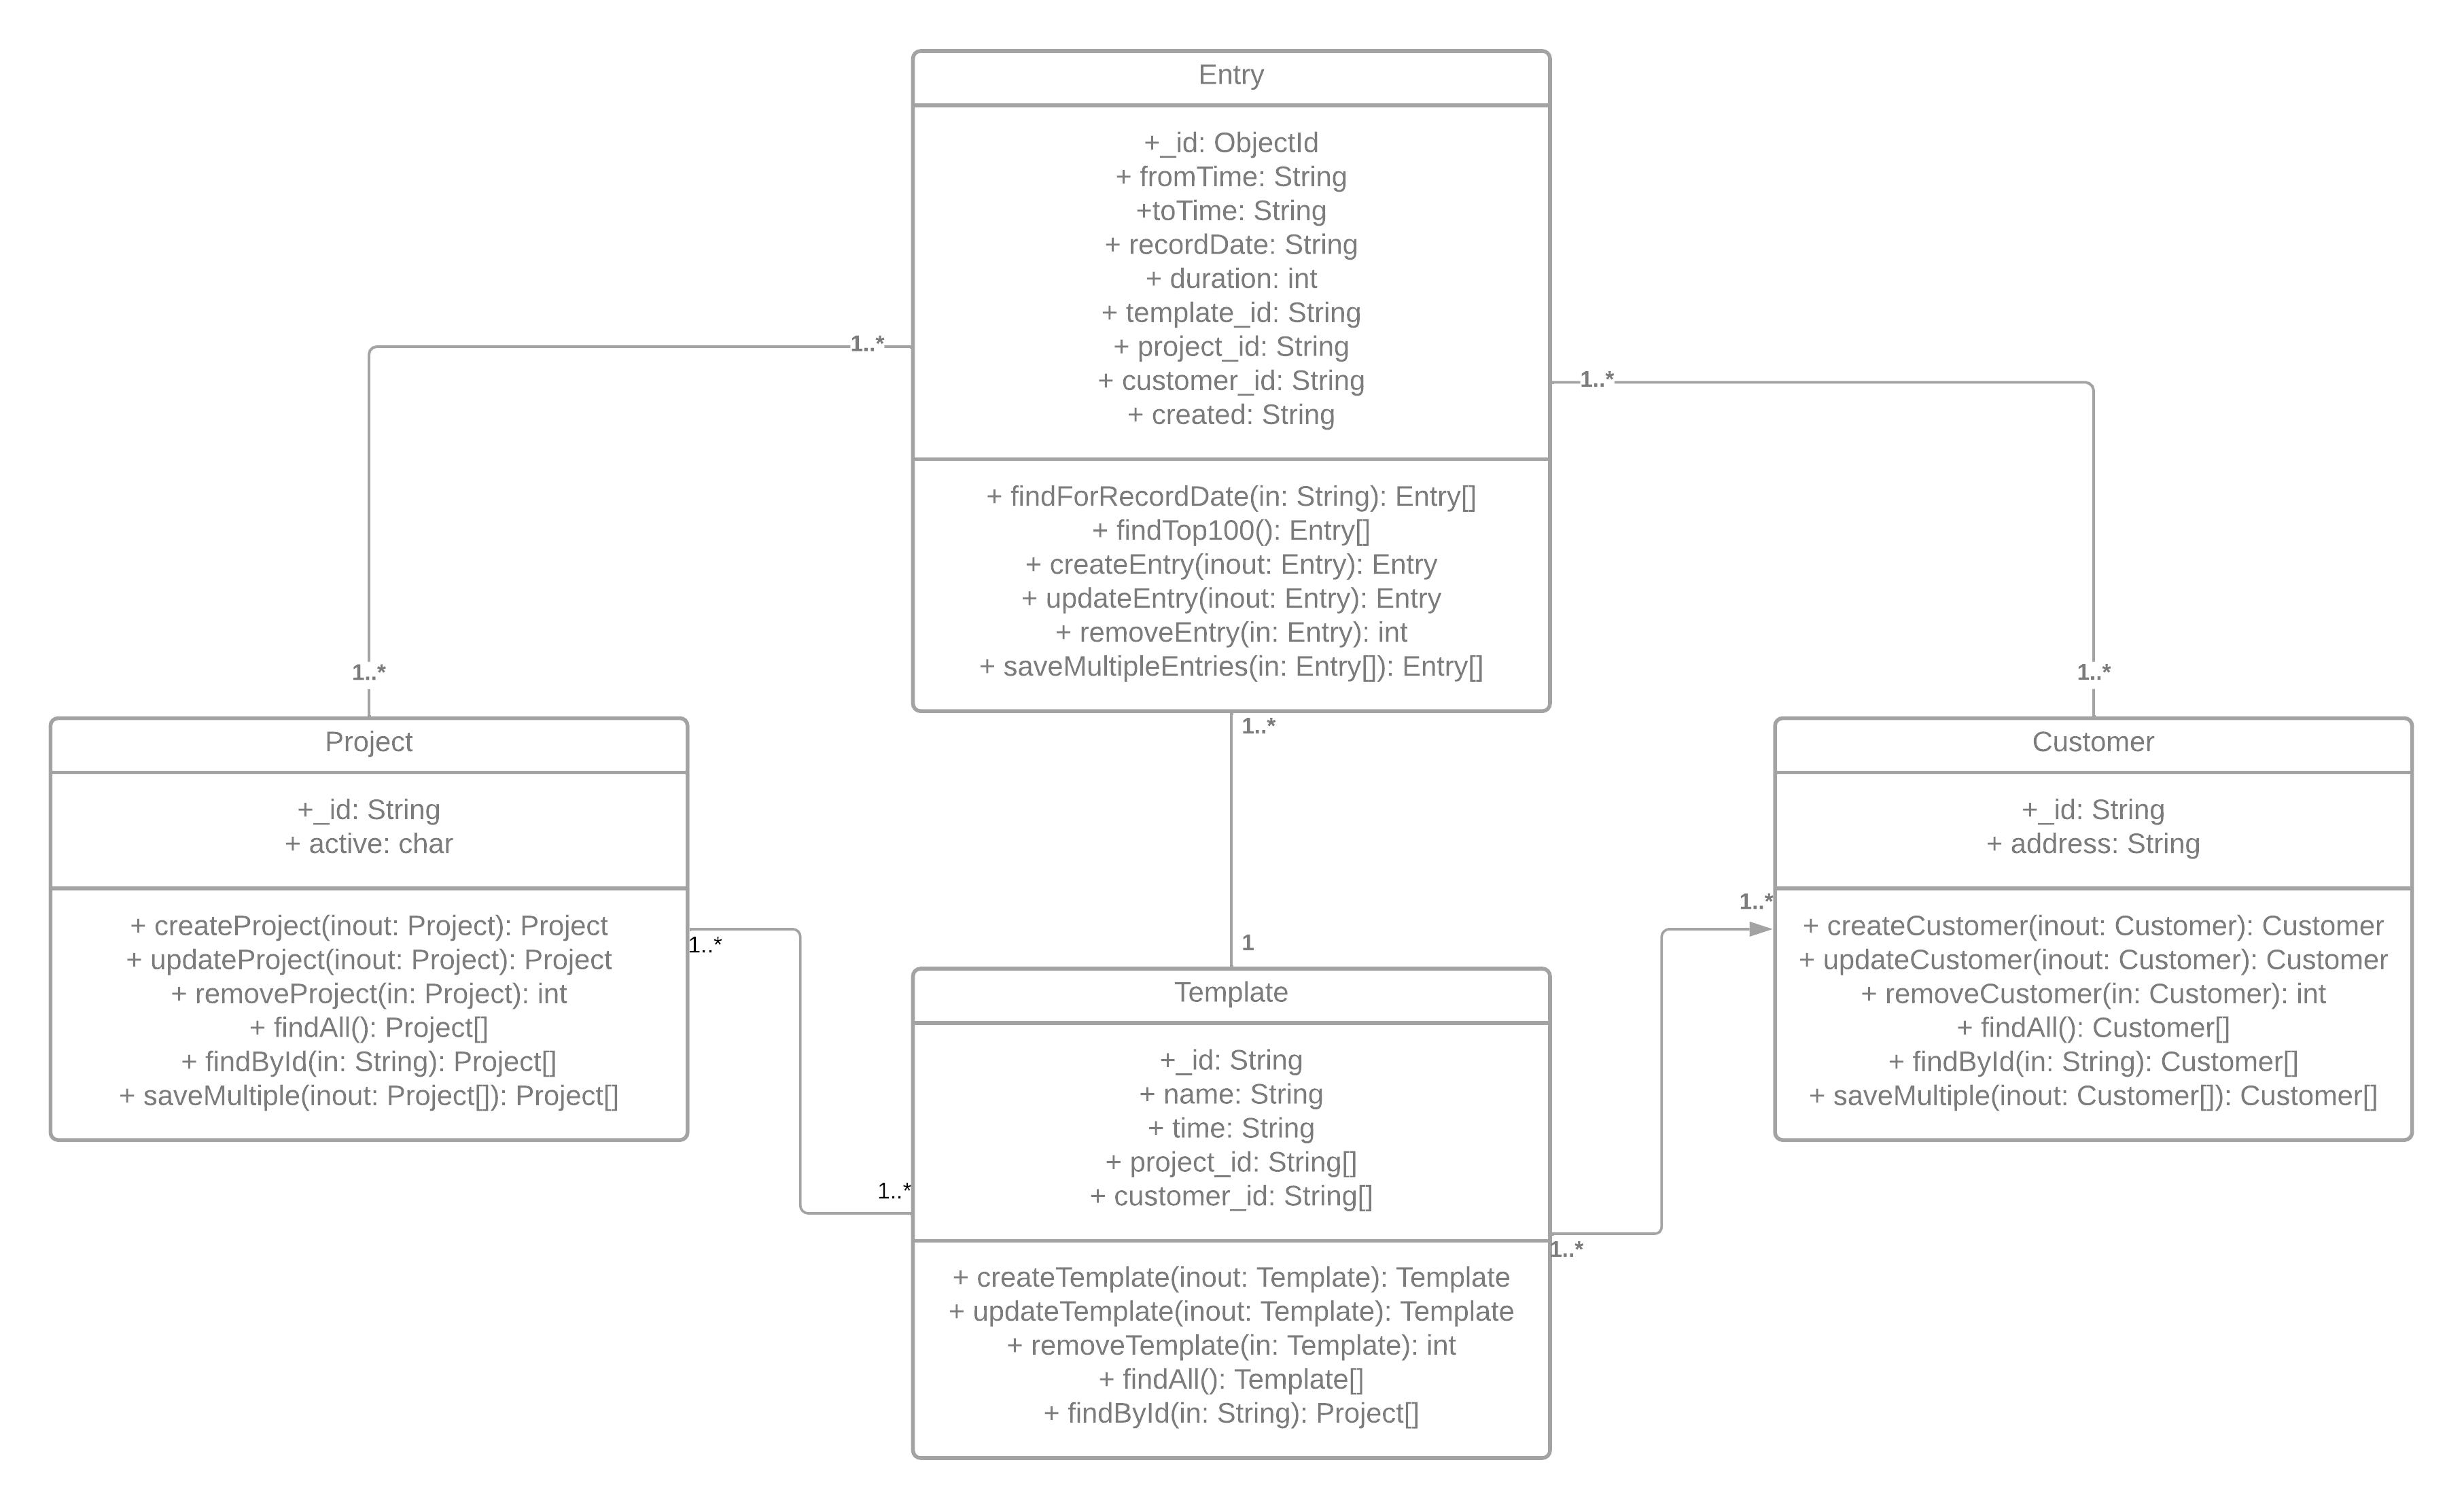
\includegraphics[width=1\textwidth]{pze-class-diagram}
\end{figure}
As seen in the figure above, all entities have similar operations and relationships. 
Each can be created, updated, and removed.
Furthermore, each offers an operation to fetch an entity based on its ID, as those are retrieved on-demand and not 
fetched eagerly.
Additionally, the Entry entity contains an operation to fetch the 100 latest entries (ordered by their recordDate attribute) in
order to return data for a local backup on each user's machine.
As the number of entries will grow once this is in use it is neither practical nor sensible to fetch all records from the database
just to make offline usage possible. 
Another unique operation of the Entry entity is fetching Entries based on their recordDate attribute. 
This is necessary as users view entries on a per-day basis.\paragraph{}
Entry, Project and Customer entities each contain an operation which allows for the creation of multiple of their respective entities.
This is to facilitate the offline functionality where users can create entities while not connected to the back-end API. 
Said entities are saved locally and once connection is restored, they are posted to the back-end and persisted.\paragraph{}
An instance of a template always references at least one customer and project, meaning that each entry which always references exactly one template 
always references at least one project and customer. 
One template can of course be referenced by multiple entries and one template can reference multiple project and vice-versa.
On the database level, a template holds an array of project and customer IDs as references.
The IDs of customer and project entities are a string representation of their given name as those have to be unique.\paragraph{}
\begin{figure}[H]
  \centering
  \label{fig:pze-component-diagram}
  \caption{A schematic overview of the application components, simplified.}
  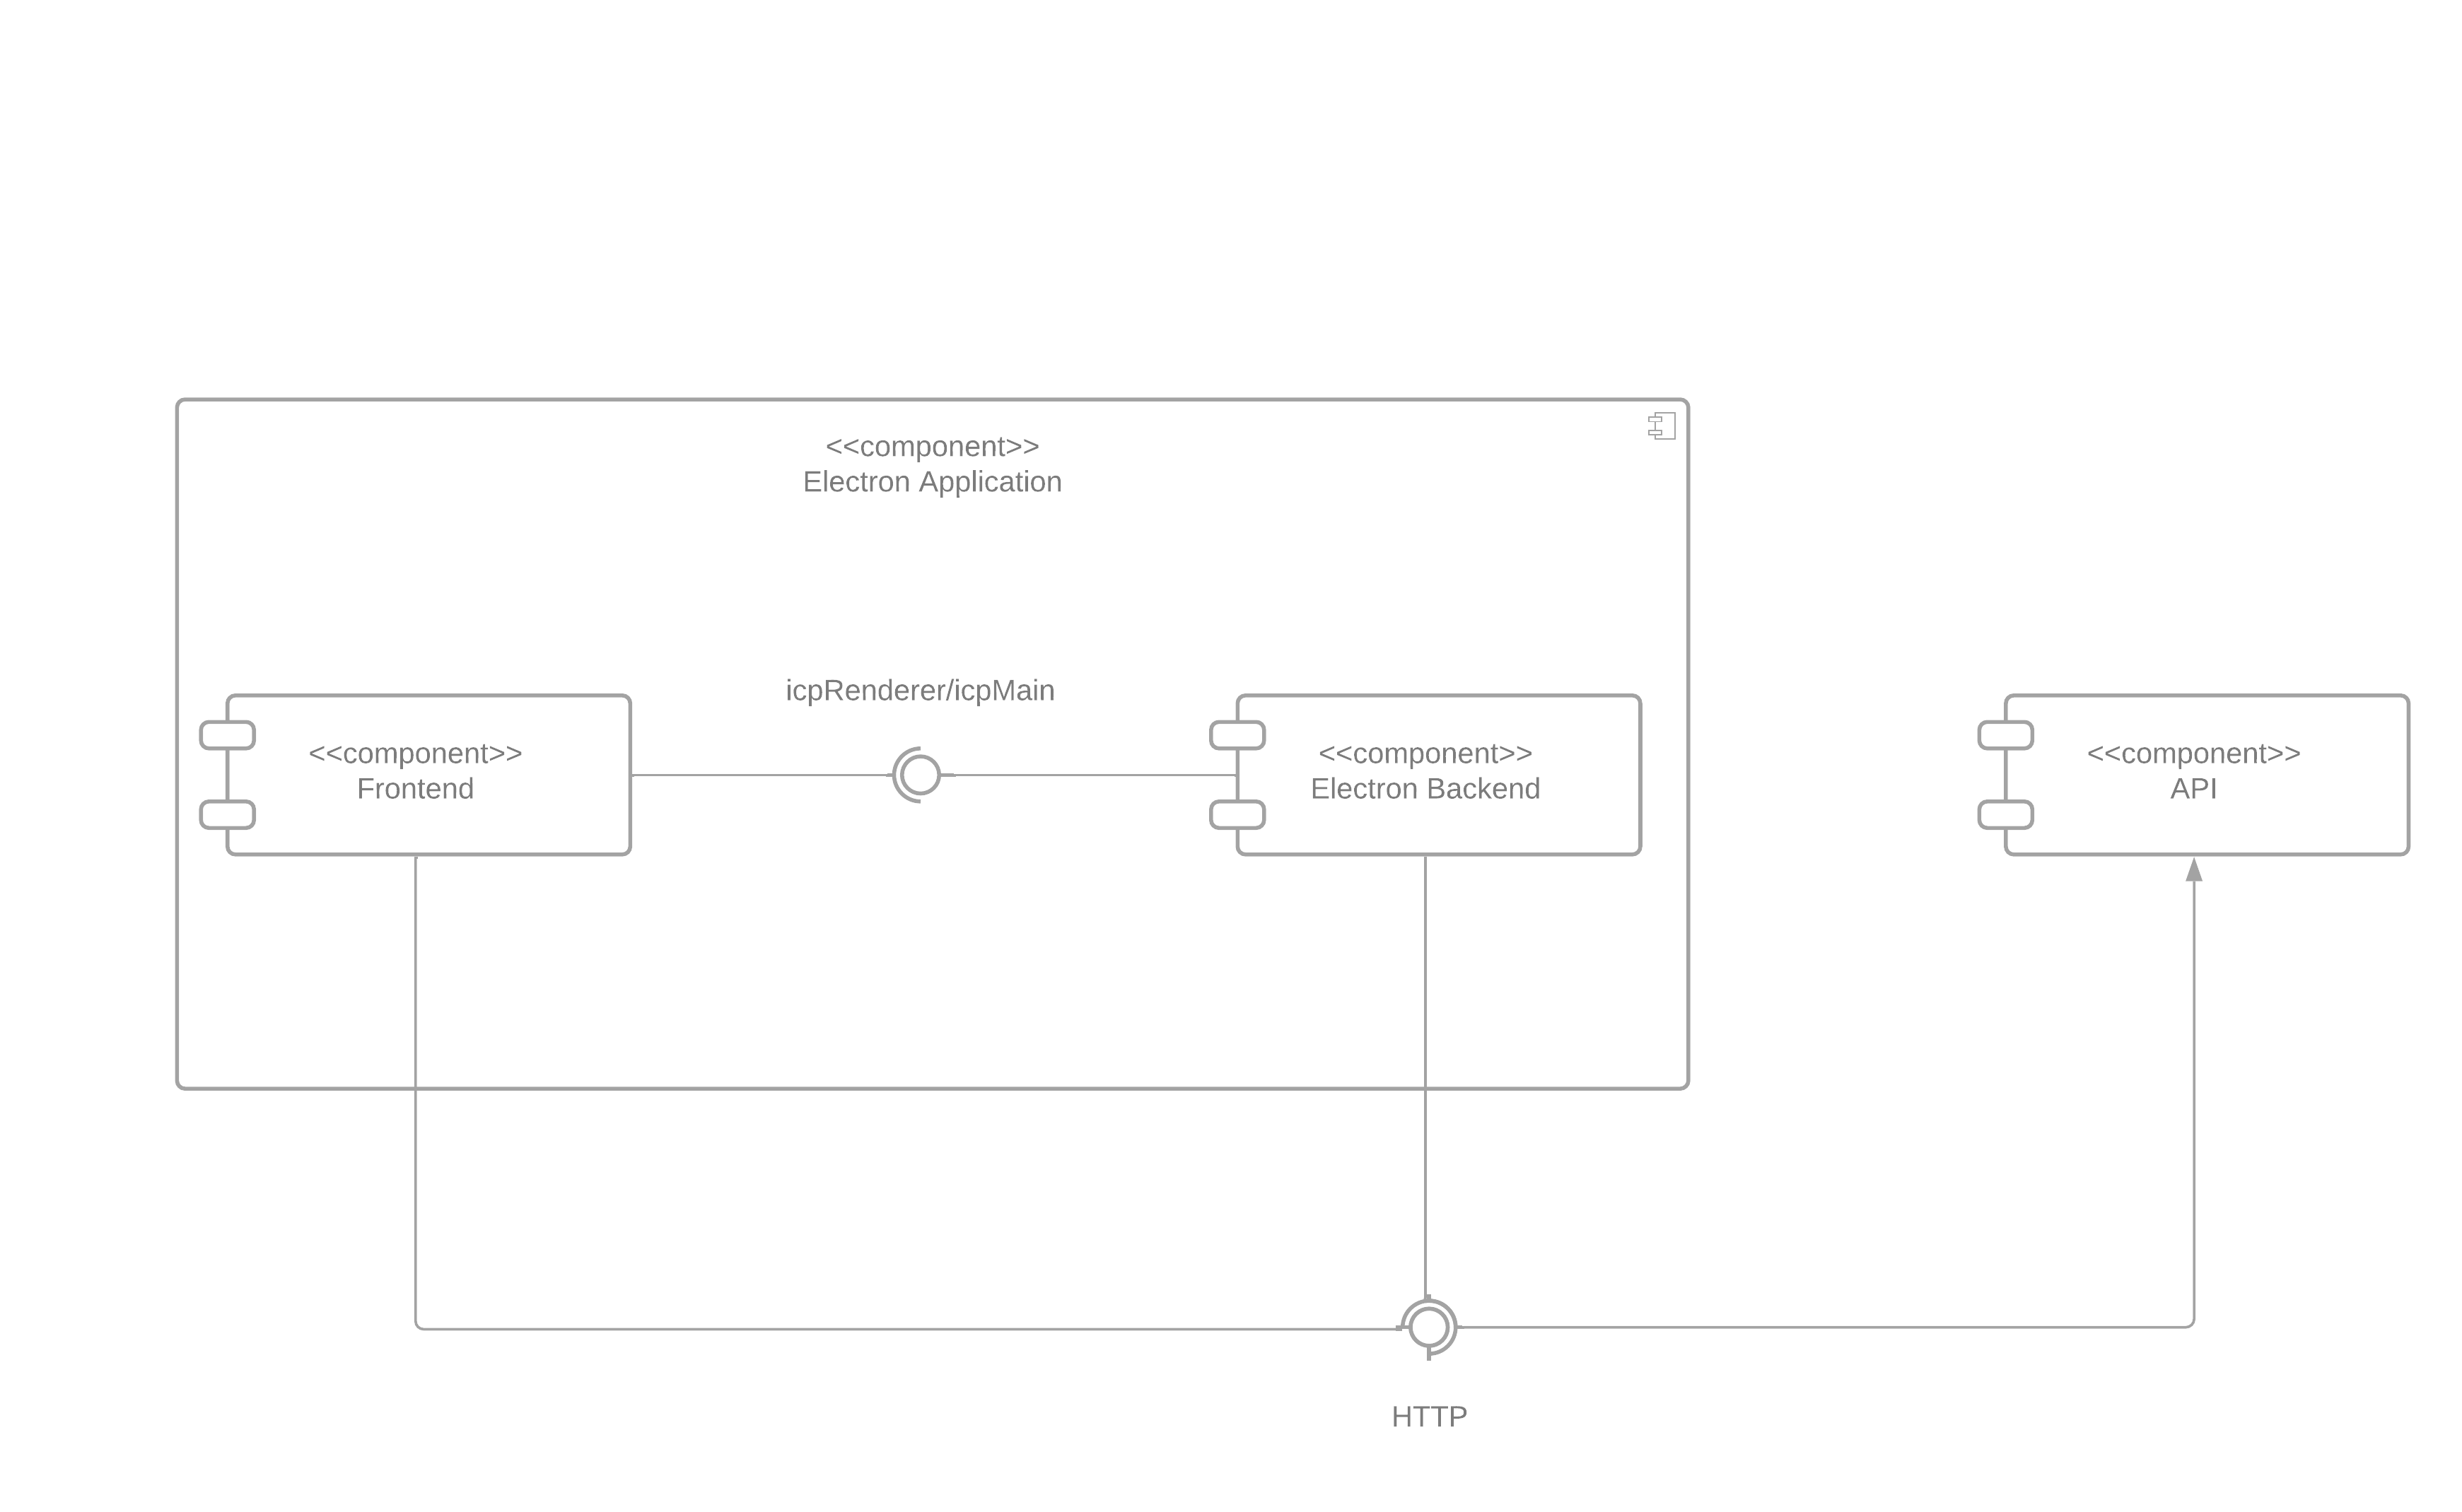
\includegraphics[width=1\textwidth]{pze-component-diagram}
\end{figure}
The above figure shows a simplified overview of the project's components. 
For the sake of illustration some implementation details have been omitted, such as the details of the database implementation in the 
back-end API.
In essence there are two ways the front-end can communicate with a data source:
Either over HTTP requests with directly the back-end or through the icpMain and icpRenderer processes with the Electron-provided back-end.
The details of this implementation will be discussed in a later chapter. 
To further illustrate the interaction between the application's components, see the following sequence diagram which illustrates
the workflow of creating an entry. 
\begin{figure}[H]
  \centering
  \label{fig:pze-sequence-diagram}
  \caption{A sequence diagram of the Create Entry use case.}
  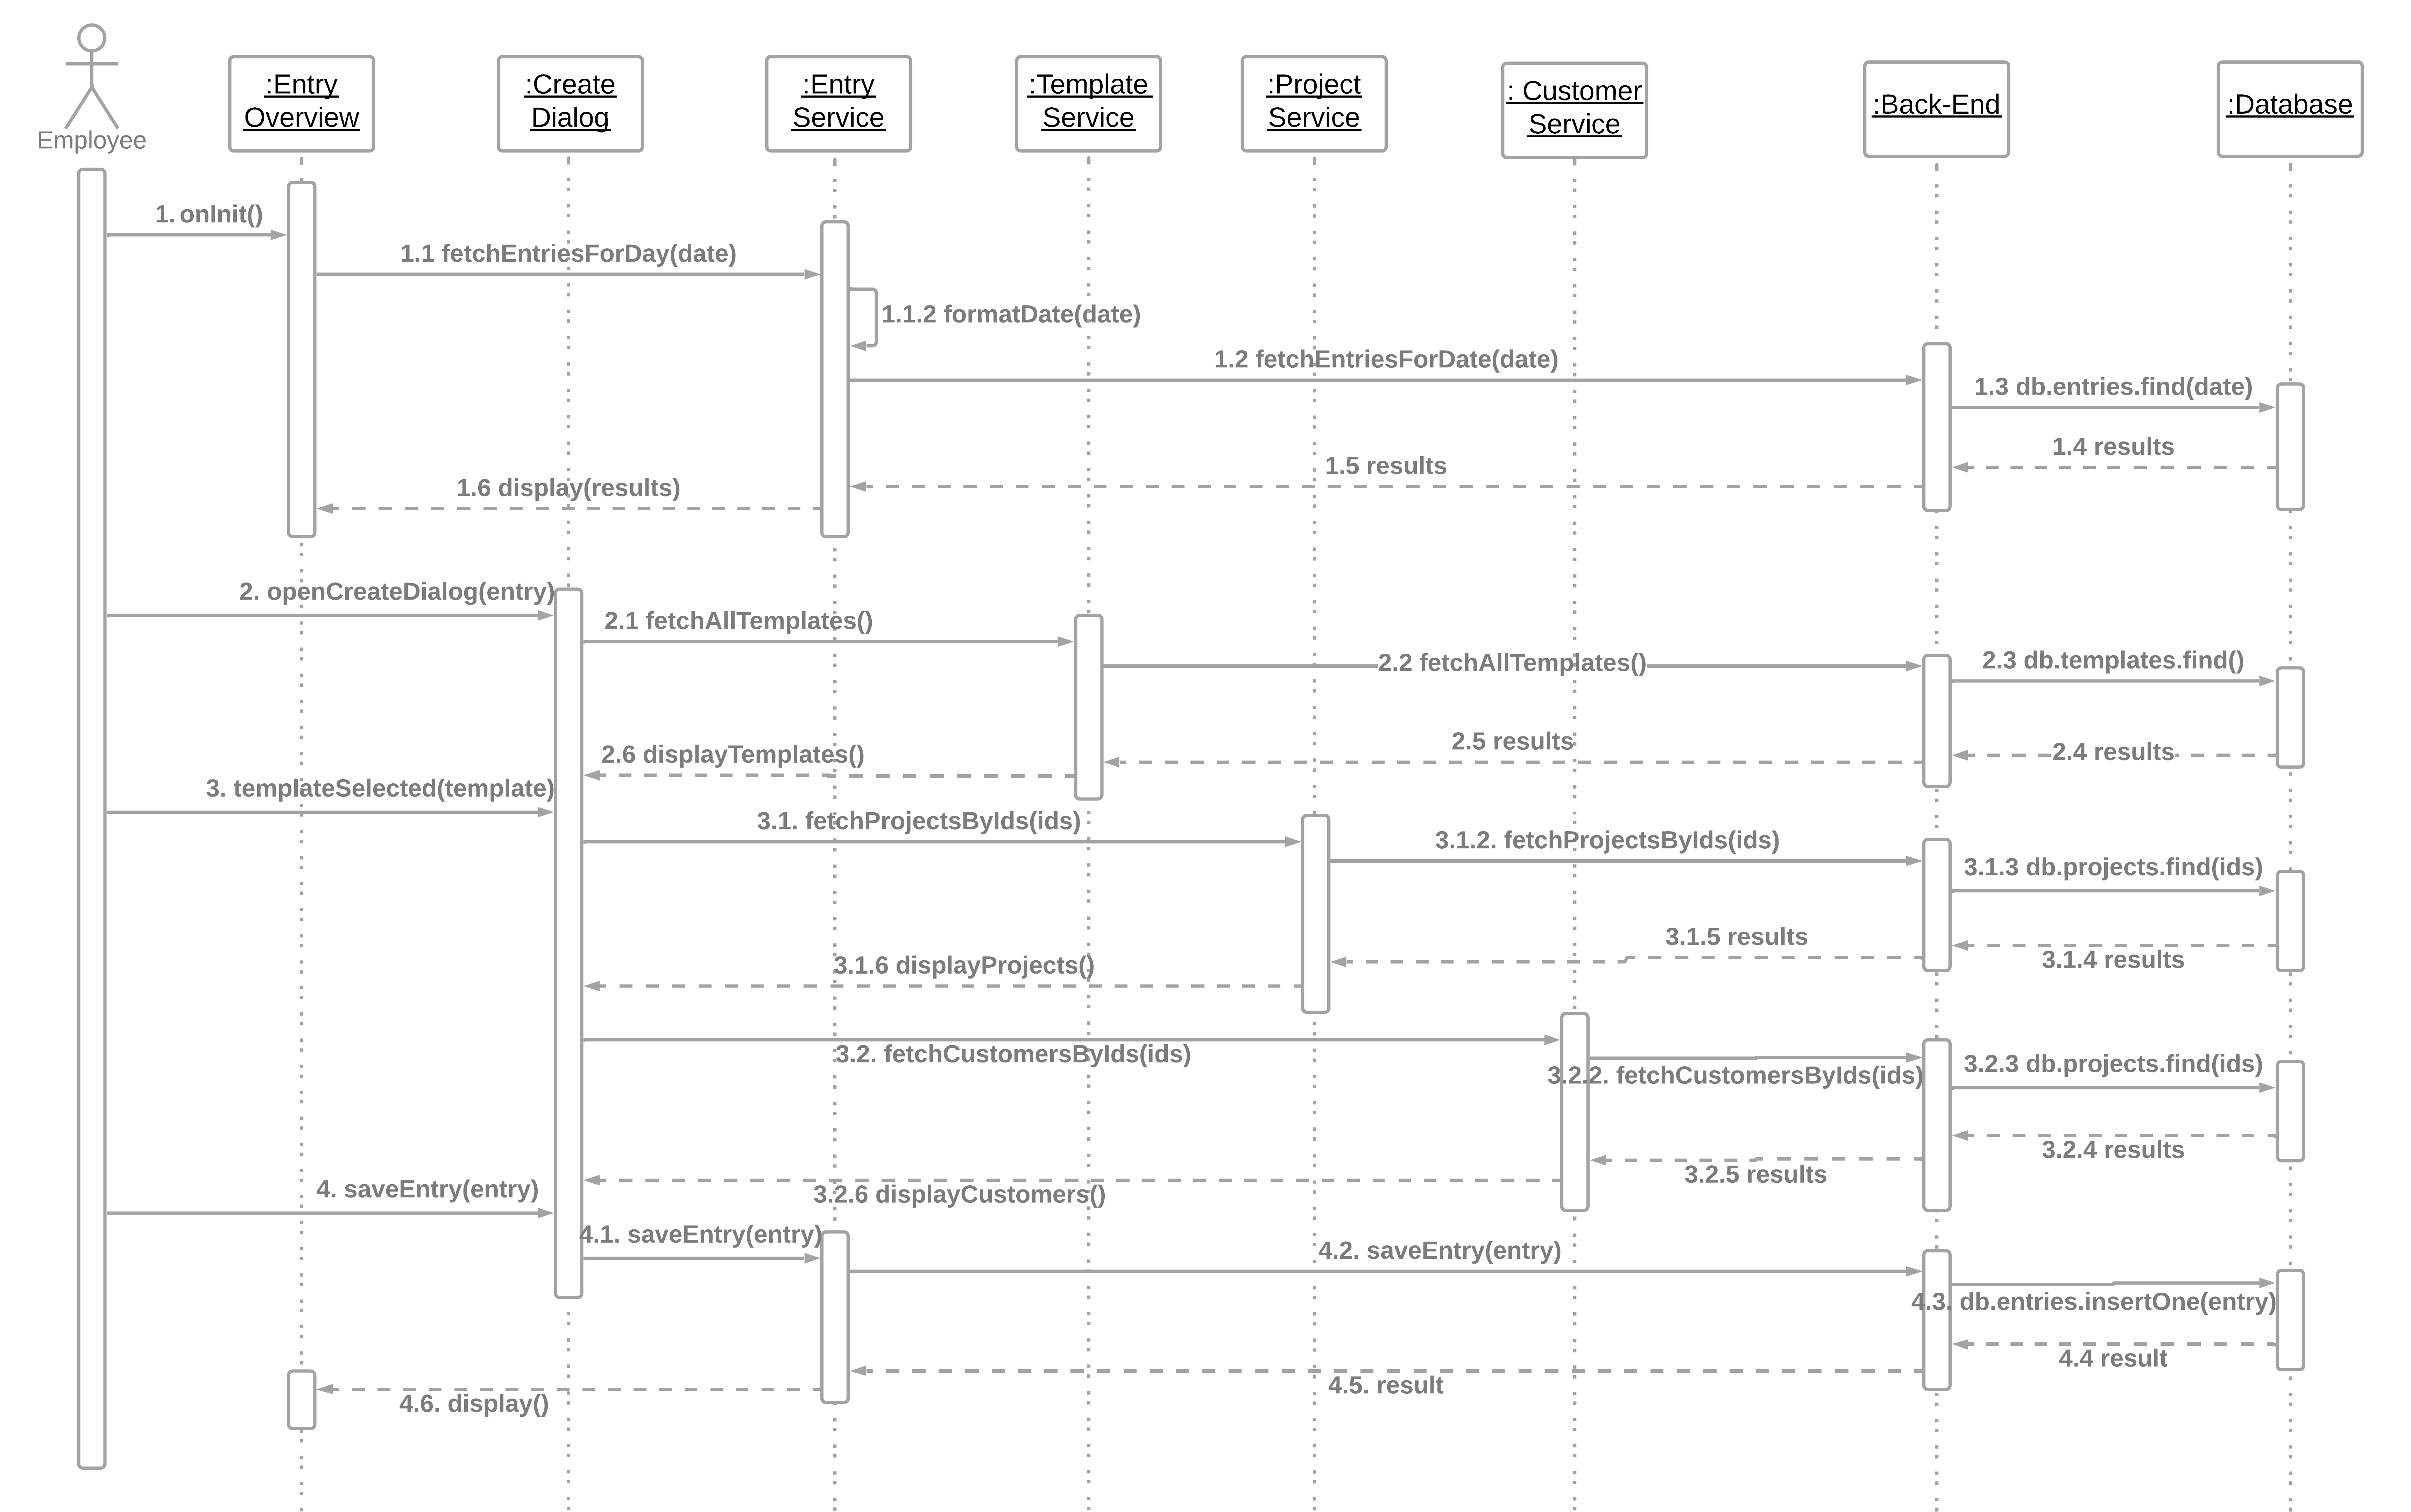
\includegraphics[width=1\textwidth]{pze-sequence-diagram}
\end{figure}
After the user has started the application they will find themselves on the entry overview which lists all entries for the selected day.
This causes a request to the back-end to fetch all entries for the specified day. 
Once the user opens the create dialog all templates are fetched and displayed to the user to choose from. 
When the user chooses a template the projects and customers defined in the selected template are fetched from the back-end. 
After the user has entered all other necessary data they can save the newly created entry which sends the object to the back-end 
and persists it in the database. 
This is an illustration to show what the workflow behind user creation of an entry looks like and how 
entries, templates, projects and customers all work in accordance.